\documentclass[12pt]{exam}
\usepackage[utf8]{inputenc}		% Caracteres latinos
\usepackage[spanish]{babel}		% Idioma español
\usepackage{geometry}			% Organizar el documento
\usepackage{graphicx}			% Incluir gráficos
\usepackage{makecell}			% Para personalizar las celdas de una tabla
\usepackage[nohdr]{mathexam}	% Añadimos el paquete mathexam (sin header)
\usepackage{amsmath}
\usepackage{amsfonts}
\usepackage{amssymb}
\usepackage{mathtools}
\usepackage{tikz,pgfplots}
\usepgfplotslibrary{polar}
\usepackage[shortlabels]{enumitem}
 \renewcommand{\baselinestretch}{1.5}
\usepackage{mathtools}
\usepackage{bm}
\usepackage{esvect}
\usepackage[fleqn]{mathtools}
\usepackage{relsize}
\usepackage{multirow}
\usepackage{multicol}
\usepackage[document]{ragged2e}
 \usepackage{textpos}
\usepackage{tcolorbox}
\usepackage{hyperref}
\usepackage{mathdesign}

%\usepackage[]{mathptmx}        % A free version o Times Roman with mathematical symbols
%\usepackage{pzc}               % fuente cursiva (conjuntos) Zapf Chancery
%\usepackage{showframe}
%\usepackage{lipsum}

% DOCUMENTACIÓN DE LA CLASE EXAM
% http://ftp.inf.utfsm.cl/pub/tex-archive/macros/latex/contrib/exam/examdoc.pdf
% DOCUMENTACIÓN DE LA CLASE MATHEXAM
% http://ctan.dcc.uchile.cl/macros/latex/contrib/mathexam/doc/mathexam.pdf

% Definimos la geometría de la primera página
\geometry{
	a4paper,                    % Tamaño del documento
	hmargin = {1.7cm, 1.6cm}, 	% Margen horizontal izquierdo, derecho
	vmargin = {1cm, 1cm},	    % Margen vertical superior, inferior
	headsep = 4mm,				% Separación entre el encabezado y el texto
	head = .2cm,				% Tamaño del encabezado
	% marginparsep = 5mm, 		% Seperación entre las notas y el texto
	% marginpar = 1.5cm,		% Tamaño de las notas
	includeall,                 % incluye el encabezado, footer y notas dentro del tamaño del documento
	nomarginpar,	            % Elimina las notas
	foot = 1cm,                 % Tamaño del footer
	twoside,                	% Habilita el modo de impresión a doble cara
}

\selectlanguage{spanish}        % Selecciona el idioma
\spanishdecimal{.}

%\pagestyle{headandfoot}         % Nuestro examen tendrá encabezado y pié

% DEFINIMOS EL ENCABEZADO
%\header{
%\begin{tabular}{l c c c l}
%            \makecell{\includegraphics[height=2.5cm]{logo.png}} &
%            \makecell{\textbf{IPEA 215} \\Raúl Scalabrini Ortiz} &
%            \makecell{Examen} &
%            \makecell{Curso\\1er Año} &
%             \makecell[l]{Apellido y %Nombre:\enspace\makebox[2in]{\hrulefill}\\Fecha: \today}
%        \end{tabular}}{}{}

% DEFINIMOS EL PIE
%\rfoot{Página \thepage\ de \numpages}
\newcommand{\iuni}{\pmb{\hat{\imath}}}
\newcommand{\juni}{\pmb{\hat{\jmath}}}
\newcommand{\kuni}{\pmb{\hat{k}}}
\renewcommand{\sin}{\,\text{sen}\,}

% DOCUMENTO
\begin{document}

\centering


\Large 
\textbf{\huge Tarea 5\\ \large Ecuaciones lineales no homogéneas}

\small
Fecha de entrega domingo 5 de Diciembre
\vskip10pt
% \flushleft
% \begin{tcolorbox}
% LEE ANTES DE COMENZAR LA TAREA
% \begin{enumerate}
%     \item Se califica sobre 10 por lo que es posible obtener 13 si se realizan también los ejercicios opcionales.
%     \item El ejercicio opcional puede sustituir a uno y solo uno de los ejercicio del bloque previo.
%     \item Subir el archivo en \textbf{PDF} a la plataforma con las páginas numeradas.

% \end{enumerate}
% \end{tcolorbox}
\normalsize

\pointpoints{punto}{puntos}
\pointformat{\bfseries\boldmath(\thepoints)}
\vskip10pt

    
    \begin{questions}
     % 1 % Nagle S4.4 e9,16,19  S4.5 e34 
     \question% 
     Determina una la solución particular de las siguientes ecuaciones diferenciales:
     \begin{enumerate}[a)]
         \item $y''+3y=-9$
         \item $\theta''(t)-\theta(t)=t\sen t$
         \item $4y''+11y'-3y=-2te^{-3t}$
         \item $y''+5y'+6y=\sen t-\cos 2t$
     \end{enumerate}


     % 2 % Nagle S4.4 e34,36  
     \question% 
     Usa el método de coeficientes indeterminados para hallar una solución particular:
     \begin{enumerate}[a)]
     	\item	$2y'''+3y''+y'-4y=e^{-t}$
        \item	$y^{IV}-3y''-8y=\sen t$
     \end{enumerate}

     
     % 3 % Nagle S4.5 e1
     \question% 
     Dada la solución $y_1(t)=\cos t$ de la ecuación $y''-y'+y=\sen t$ y que $y_2(t)=e^{2t}/3$ es solución de $y''-y'+y=e^{2t}$; usa el principio de superposición para determinar soluciones de las siguientes ecuaciones diferenciales:
     \begin{enumerate}[a)]
     	\item	$y''-y'+y=5\sen t$
        \item	$y''-y'+y= \sen t-3e^{2t}$
        \item	$y''-y'+y=4\sen t+18e^{2t}$
     \end{enumerate}


     % 4 % Nagle S4.5 e18,20,22
     \question% 
     Determina una solución general:
     \begin{enumerate}[a)]
     	\item	$y''-2y'-3y=3t^2-5$
        \item	$y''(\theta)+4y(\theta)=\sen\theta-\cos\theta$
        \item	$y''(x)+6y'(x)+10y(x)=10x^4+24x^3+2x^2-12x+18$
     \end{enumerate}



     % 5 % Nagle S4.5 29,30
     \question%
     Determina la solución del problema con valores iniciales:
     \begin{enumerate}[a)]
        \item	$y''(\theta)-y(\theta)=\sen\theta-e^{2\theta}$;  $y(0)=1$,  $y'(0)=-1$
        \item	$y''+2y'+y=t^2+1-e^t$;  $y(0)=0$,  $y'(0)=2$
     \end{enumerate}



     % 6 % Nagle s4.5 e43
     \question% 
     Un sistema masa-resorte recibe una fuerza externa sinusoidal $g(t)=5\sen t$. La masa es igual a 1, la constante de resorte es igual a 3 y el coeficiente de amortiguamiento es igual a 4. Si la masa se coloca inicialmente en $y(0)=1/2$ y en reposo, es decir, $y'(0)=0$, determina su ecuación de movimiento.


     % 7 % Nagle S4.6 e2,3,10
     \question%
     Determina una solución general usando el método de variación de parámetros:
     \begin{enumerate}[a)]
     	\item $y´´+y=\sec t$
        \item $2x''-2x'-4x=2e^{3t}$
        \item $y''+4y'+4y=e^{-2t}\ln t$
\end{enumerate}


     
     
     % 8 % Nagle S4.6 e12,15
     \question%
     Determina una solución general para la ecuación $y''+y=3\sec t-t^2+1$.
     

     
     % 9 % Nagle S4.6 e21
     \paragraph{Ecuaciones con coeficientes variables.} El método de variación de parámetros también se aplica a ecuaciones con coeficientes variables de la forma $$a(t)y''+b(t)y'+c(t)y=g(t)$$
     
     Si $y_1(t)$, $y_2(t)$ son soluciones de la ecuación homogénea correspondiente, linealmente independientes en un intervalo $I$ y $a(t)\neq0$ en $I$, entonces la ecuación anterior tiene una solución particular de la forma $y_p(t)=v_1(t)y_1(t)+v_2(t)y_2(t)$, donde $v_1'$, $v_2'$ quedan determinadas nuevamente por las ecuaciones $y_1v_1'+y_2v_2'=0$, $y_1'v_1'+y_2'v_2'=g/a$ aunque reemplazando la constante $a$ por la función $a(t)$.
    \question% 
     Determina una solución particular de la ecuación con coeficientes variables dado $y_1$ y $y_2$ como soluciones linealmente independientes de la ecuación homogénea correspondientes para $t>0$.$$ty''-(t+1)y'+y=t^2;\quad y_1=e^t,\quad y_2=t+1$$


     % 10 % Nagle impreso 4.4 e3,5 Moya pp164 e k)
     \question%
    Mediante el método de reducción de orden, determina una segunda solución linealmente independiente a la solución dada $f$:
    \begin{enumerate}[a)]
        \item $x^2y''-2xy'-4y=0$,  $x>0$;  $f(x)=x^{-1}$
        \item $tx''-(t+1)x'+x=0$,  $t>0$;  $f(t)=e^t$
        \item $x^2y''-5xy'+8y=4x^2$;  $f(x)=x^2$
    \end{enumerate}

    %  % 11 %
    %  \question% 
     

    %  % 12 %
    %  \question% 
     
     
        \end{questions}
        \vskip30pt
  \RaggedRight
	2 PUNTOS EXTRAS %Nagle S4.7 e7,8
	
    Para deducir la ecuación del péndulo $m\theta'' +m\frac{g}{l}\sen\theta=0$, realice los pasos siguientes.
    \begin{enumerate}[a)]
        \item El momento angular de la masa del péndulo $m$ medido en torno del soporte $O$ de la figura está dado por el producto de la longitud del 	"brazo de palanca"	$l$ y el componente
del momento vectorial $mv$ perpendicular al brazo de la palanca. Muestra que esto da como resultado $$momento\,angular=ml^2\frac{d\theta}{dl}$$
		\item La torca producida por la gravedad es igual al producto de la longitud del brazo de palanca $l$ por la componente de la fuerza (vectorial) de gravedad $mg$ perpendicular al brazo de palanca.
Muestra que esto implica $$torca=-lmg\sen\theta$$
		\item Ahora usa la ley de Newton para el movimiento rotacional y deduce la ecuación del péndulo $ml^2\theta''=-lmg\sen\theta$.
        
        \item Usa el lema de la integral de la energía para mostrar que los movimientos del péndulo cumplen $$\frac{(\theta')^2}{2}-\frac{g}{l}\cos\theta=constante$$

    \end{enumerate}
    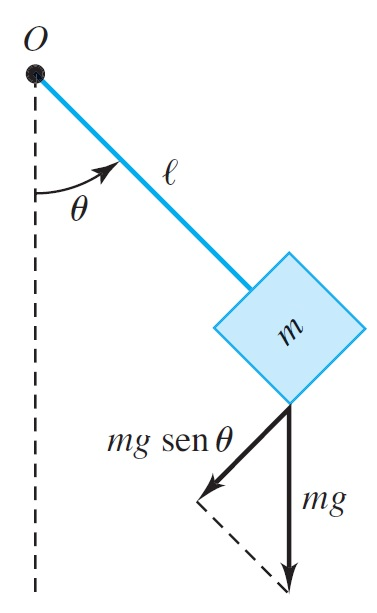
\includegraphics[scale=.5]{T5Extra.jpg}
    

    
    


 
 

 
    
%     \newpage



% Geometría para la otra carilla
\newgeometry{
	hmargin = {1.5cm, 1.5cm},
	vmargin = {5cm, 1cm},
	%nofoot,			% Elimina el pié
	nohead,			% Elimina el encabezado
	nomarginpar,	% Elimina las notas
	includeall,
}% \savegeometry{geometria_1}

\pagestyle{foot}    % El estilo de ésta página sólo constará de pié de página
\runningfooter{}{}{Página \thepage\ de \numpages}


%\lipsum[1-5]

% \restoregeometry
% \loadgeometry{geometria_1}


\end{document}
